\documentclass{magnolia}

\magtex{tex_driver={pdftex}}
\magfiche{document_nom={TP Cryptographie},
          auteur_nom={Victor Lambert},
          auteur_mail={victor.lambert@ens-cachan.org}}
\magcours{cours_matiere={informatique},
          cours_niveau={mpsi},
          cours_chapitre_numero={2},
          cours_chapitre={TP Python}}
\magmisenpage{}
\maglieudiff{}
\magprocess


\begin{document}

%BEGIN_BOOK
La cryptographie a pour but de transformer des messages afin qu'ils ne puissent être lus
que par des personnes de confiance. Ces dernières sont les seules à connaitre le
mécanisme permettant d'effectuer la transformation inverse afin de retrouver le message
d'origine.\\

Au premier siècle de notre ère est apparu un chiffrement par substitution, connu sous le
nom de code de César, car l'empereur en a été l'un des plus assidus utilisateurs.
Le chiffrement de César consiste à assigner à chaque lettre de l'alphabet une
autre lettre, résultant du décalage de l'alphabet d'un certain nombre de lettres. Par exemple, avec le décalage suivant
\begin{center}
\begin{tabular}{|*{26}{c|}}
\hline
a&b&c&d&e&f&g&h&i&j&k&l&m&n&o&p&q&r&s&t&u&v&w&x&y&z\\
\hline
f&g&h&i&j&k&l&m&n&o&p&q&r&s&t&u&v&w&x&y&z&a&b&c&d&e\\
\hline
\end{tabular}
\end{center}
le texte \verb_"vous suivez le cours de python"_ devient
\verb_"atzx xznaje qj htzwx ij udymts"_. Pour décoder le message, il suffit de connaitre
la clé, c'est-à-dire la lettre qui correspond à la lettre \verb_"a"_. Dans l'exemple
ci-dessus, la clé est donc \verb_"f"_.\\

Le but de ce TP est d'écrire un programme permettant de coder un message par cette
méthode, puis un autre permettant de décoder ce message. On verra aussi comment attaquer
cette méthode de cryptage, c'est-à-dire comment un pirate peut intercepter le message
et retrouver la clé du cryptage afin de le décoder. 

\section{Codage et décodage par la méthode de César}

\begin{questions}
\question Écrire une fonction \verb_ordre(c: str) -> int_ qui à une lettre de l'alphabet
  latin associe sa position dans l'alphabet. Par exemple, à la lettre \verb_"a"_,
	la fonction \verb_ordre_ associera l'entier 0 et à la lettre \verb_"z"_ elle associera
	l'entier 25. On utilisera pour cela la fonction \verb_ord_ de Python.
\question Écrire une fonction réciproque \verb_lettre(n: int) -> str_  qui à l'entier
  $n\in\intere{0}{25}$ associe la lettre associée. Par exemple \verb_lettre(2)_ doit renvoyer
	\verb_"c"_.
\question Écrire une fonction \verb!est_lettre_alphabet(c: str) -> bool! qui renvoie
  \verb_True_ si \verb_c_ est une lettre de l'alphabet latin et \verb_False_ sinon.
	Par exemple \verb!est_lettre_alphabet("a")! va renvoyer \verb_True_ et
	\verb!est_lettre_alphabet(".")! va renvoyer \verb_False_.
\question Écrire une fonction \verb_code(m: str, c: str) -> str_ qui au message \verb_m_
  et à la clé \verb_c_ associe le message obtenu en utilisant le codage de
	César. Par exemple, l'appel \verb_code("lazos rocks", "c")_ doit renvoyer
	\verb_"ncbqu tqemu"_.
\question Écrire la fonction \verb_decode(s: str, c: str) -> str_ qui effectue
  la transformation inverse. L'appel à la fonction
	\verb_decode("ncbqu tqemu", "c")_ doit renvoyer \verb_"lazos rocks"_.
\end{questions}

\section{Déterminer la clé}

On intercepte un message codé par le chiffrement de César dont on ignore la clé.
On veut déterminer une méthode automatique qui nous donnera la clé et le message original.
Pour cela, nous allons exploiter l'idée que, dans une langue donnée, la fréquence
d'apparition de chacune des lettres de l'alphabet n'est pas la même.\\

Au début du fichier \texttt{crypto.py}, il y a une liste \verb_g_ des fréquences
d'apparition des lettres de l'alphabet en français. Par exemple, la lettre \verb_"a"_
apparaît, dans un texte comportant  $100$ caractères alphabétiques, en moyenne $8.4$
fois. Pour casser le codage de César, nous allons comparer cette liste \verb_g_
à la liste \verb_f_ des fréquences obtenues dans le texte encrypté.

\begin{questions}
\question Écrire une fonction \verb_frequence(m: str) -> list[float]_, qui a pour argument
  un message \verb_m_, et qui renvoie une liste de $26$ éléments contenant la fréquence 
	d'apparition de chacune des lettres de l'alphabet dans le message \verb_m_. Pour cela
	on commencera par initialiser une liste de 26 zéros à l'aide de l'instruction
	\verb_f = 26 * [0]_.
\enonce Pour trouver la clé, on va faire \og tourner \fg le tableau \verb_f_ des fréquences
  d'apparition de notre message pour le faire coïncider le mieux possible avec le tableau
	\verb_g_ des fréquences des lettres dans la langue française. 
\question Écrire une fonction \verb_distance(f: list[float], g: list[float], i: int) -> float_
  qui a pour argument deux listes de fréquences \verb_f_ et \verb_g_ ainsi qu'un décalage
	$i\in\intere{0}{25}$ et qui renvoie la distance
  \[d_i\defeq \sum_{j=0}^{25}\abs{g_j-f_{i+j\ ({\rm mod}\ 26)}}\]
\question Écrire une fonction \verb!indice_minimum_distance(m: str, g: list[float]) -> int!
  qui a pour argument un message \verb_m_ et qui renvoie l'entier  \verb_i0_ tel que
	\[d_{i_0}=\min\ensim{d_i}{i\in\intere{0}{25}}.\]
\question Écrire une fonction \verb!decrypte(m: str, g: list[float]) -> str! qui a pour
  argument un message \verb_m_ et qui renvoie le message en clair.
\question Tester la fonction précédente sur le message codé
  \verb_message_ présent dans le fichier distribué.
	%dans \texttt{messages.py}.
\end{questions}

%\section{Amélioration}
%
%Nous allons faire en sorte que la méthode de codage fonctionne sur des textes écrits avec des majuscules et des accents.
%\smallskip
%
%\emph{Remarques}: 
%\begin{itemize}
%\item[\textbullet] On supposera, dans la suite, que les majuscules ne sont pas accentuées.
%\item[\textbullet] On n'utilisera pas de fonction prédéfinie en python pour répondre aux question suivantes.
%\end{itemize}
%\smallskip
%
%\begin{enumerate}
%\item \'Ecrire une fonction \texttt{enleve\_majuscules} d'argument une chaîne \texttt{texte} qui renvoie la même chaîne en transformant les majuscules en minuscules.
%
%\item \'Ecrire une fonction \texttt{enleve\_accents} d'arguments une chaîne \texttt{texte}  qui renvoie la même chaîne en enlevant les accents et en remplaçant les ç par des c.
%
%\item Avec les fonctions suivantes, transformez \texttt{message4} pour ne plus avoir ni majuscules, ni accents. Proposez un codage du message obtenu avec la clé de votre choix puis effectuer un décodage automatique.
%\end{enumerate}


\section{Chiffre de Vigenère}

L'idée de Vigenère est d'utiliser un chiffre de César, mais où le
décalage utilisé change de lettre en lettre. Pour cela, on utilise une table composée de
26 alphabets, écrits dans l'ordre, mais décalés de ligne en ligne d'un caractère. On
écrit encore en haut un alphabet complet, pour la clé, et à gauche, verticalement, un
dernier alphabet, pour le texte à coder. 

\begin{center}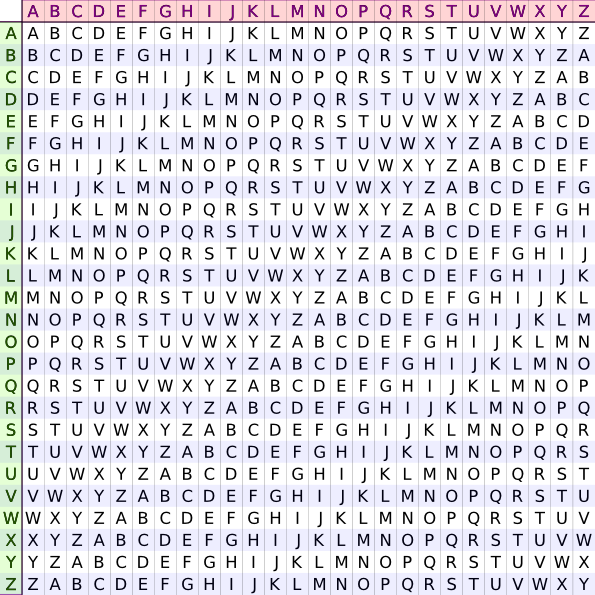
\includegraphics[width=7cm]{../../Commun/Images/python-tps-vigenere.png}\end{center}

Pour coder un message, par exemple \verb_"cryptographie de vigenere"_, on choisit une clé
qui sera un mot de longueur arbitraire ; prenons \texttt{mathweb}. On écrit ensuite cette
clé sous le message à coder. Dans cette partie, on supposera que le message à coder ne comporte que
des lettres de l'alphabet et pas de point, de virgule, ni d'espace. On répète la clé
aussi souvent que nécessaire pour que sous chaque lettre du message à coder, on trouve
une lettre de la clé.
\begin{center}
\begin{tabular}{|*{25}{c|}}
\hline
c&r&y&p&t&o&g&r&a&p&h&i&e&d&e&v&i&g&e&n&e&r&e\\
\hline
m&a&t&h&w&e&b&m&a&t&h&w&e&b&m&a&t&h&w&e&b&m&a\\
\hline
\end{tabular}
\end{center}

\noindent
Pour coder, on regarde dans le tableau l'intersection de la ligne de la lettre à coder avec
la colonne de la lettre de la clé. Dans notre exemple, on commence par coder la lettre
\verb_"c"_ . La clé est donnée par la lettre  \verb_m_. On regarde dans le tableau 
l'intersection de la \og ligne \fg \verb_c_ et de la \og colonne\fg \verb_m_. Ainsi ce
\verb_"c"_ sera codé par \verb_"o"_. Ensuite, on code la lettre  \verb_"r"_, dont la clé est
\verb_a_. La lecture du tableau donne la lettre  \verb_"r"_ (ligne \verb_r_ et colonne
\verb_a_). Ainsi de suite. Notre message sera codé par \verb_"orrwpshdaioei eq vbnarfde"_. 

\begin{center}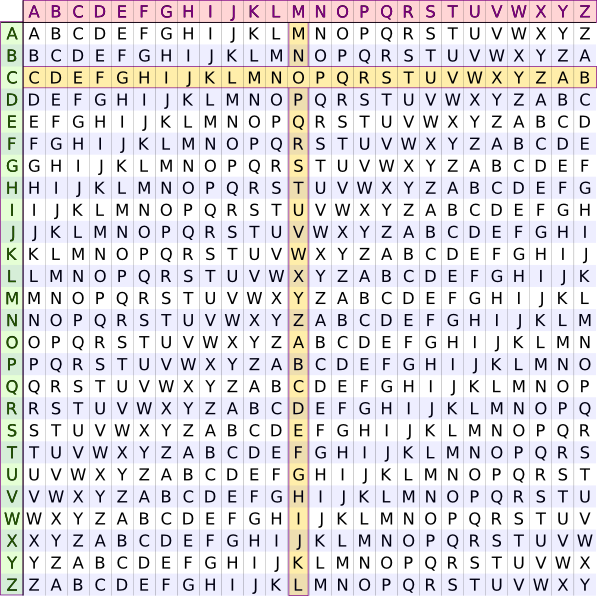
\includegraphics[width=7cm]{../../Commun/Images/python-tps-vigenere2.png}\end{center}

L'intérêt par rapport au codage de César est qu'une même lettre sera codée par
plusieurs lettres différentes ; par exemple ici \verb_"e"_ est codé par \verb_"i"_,
\verb_"q"_, \verb_"a"_, \verb_"f"_ et \verb_"e"_.

\begin{questions}
\question Écrire une fonction \verb!code_vigenere(m: str, cle: str) -> str! d'arguments
un message en clair \verb_m_ et une clé \verb_cle_. Cette fonction renverra le message
codé selon le code de Vigenère avec la clé \verb_cle_.
\question Écrire une fonction \verb!decode_vigenere(m: str, cle:str) -> str! d'arguments
un message codé \verb_m_ selon Vigenère avec la clé \verb_cle_ . Cette
fonction renverra le message décodé.
\question Écrire une fonction \verb!decrypte_vigenere(m: str, n: int, g: list[float]) -> str! d'arguments un message codé \verb_m_ selon Vigenère, la longueur de la clé
\verb_n_ et le tableau \verb_g_ des fréquences des lettres dans la langue française. 
\question Décoder \verb!message_vigenere! qui a été codé avec la méthode de
  Vigenère, sachant que la clé possède $11$ lettres.
\end{questions}

%END_BOOK
\end{document}
